\chapter{System Design and Implementation}
\label{chap:system_design}

\section{Design goals}

The implementation of \texttt{Svg2GPU} follows a product-oriented design: parse reliably, convert deterministically, and render with explicit API boundaries.
The system is intentionally modular so that parser, geometry logic, and renderer can evolve independently.

Core design goals are:

\begin{itemize}
\item predictable parser output for supported SVG input,
\item clear style normalization rules,
\item geometry conversion separated from XML concerns,
\item practical rendering integration for browser environments,
\item reproducible testing and documentation support.
\end{itemize}

\section{Architecture overview}

At project level, the solution has two components:

\begin{enumerate}
\item \textbf{Core library} (\texttt{svg2gpu})
\item \textbf{Client application} (\texttt{client})
\end{enumerate}

The library implements parsing, typing, style handling, and rendering utilities.
The client offers playground-based interactive testing and documentation exposure.

\subsection{Layered architecture for F1 and F2}

The first two evaluated functionalities are intentionally located at the beginning of the pipeline.
F1 validates the path parsing boundary, while F2 validates the style and color normalization boundary.
These two functions are tested first because geometry conversion and rendering depend on stable typed input.

\begin{figure}[htbp]
\centering
\footnotesize
\renewcommand{\arraystretch}{1.45}
\begin{tabular}{|>{\centering\arraybackslash}p{3.1cm}|>{\centering\arraybackslash}p{3.0cm}|>{\centering\arraybackslash}p{3.0cm}|>{\centering\arraybackslash}p{3.0cm}|}
\hline
\textbf{Test entry} & \textbf{Public API} & \textbf{Parser methods} & \textbf{Output checked} \\
\hline
F1 test suite &
SVG parser class &
path command parser &
typed command list \\
\hline
Jest assertions &
main parse method &
element parser and style parser &
path object or safe rejection \\
\hline
\end{tabular}

\vspace{0.35cm}
\textbf{Flow:}
F1 tests $\rightarrow$ SVG parser $\rightarrow$ path and element parsing $\rightarrow$ typed commands, normalized style, or empty result for invalid input.
\caption{Layered/class interaction diagram for F1: SVG path parsing pipeline}
\label{fig:f1_architecture}
\end{figure}

\begin{figure}[htbp]
\centering
\footnotesize
\renewcommand{\arraystretch}{1.45}
\begin{tabular}{|>{\centering\arraybackslash}p{3.0cm}|>{\centering\arraybackslash}p{3.0cm}|>{\centering\arraybackslash}p{3.3cm}|>{\centering\arraybackslash}p{3.0cm}|}
\hline
\textbf{Test entry} & \textbf{Public API} & \textbf{Normalization logic} & \textbf{Output checked} \\
\hline
Color parser test suite &
color parse method &
HEX, RGB/RGBA, HSL/HSLA validators &
RGBA color array \\
\hline
Jest assertions &
HSL conversion helper &
named colors, transparent, none &
rejection for invalid colors \\
\hline
SVG parser style consumer &
common style parser &
defaults for missing style fields &
normalized style object \\
\hline
\end{tabular}

\vspace{0.35cm}
\textbf{Flow:}
F2 tests $\rightarrow$ color parser $\rightarrow$ validators, converters, and defaults $\rightarrow$ normalized RGBA/style values or safe rejection.
\caption{Layered/class interaction diagram for F2: style and color normalization pipeline}
\label{fig:f2_architecture}
\end{figure}

\begin{table}[htbp]
\centering
\caption{What F1 and F2 test in the architecture}
\label{tab:f1_f2_architecture_focus}
\begin{tabular}{>{\raggedright\arraybackslash}p{1.4cm} >{\raggedright\arraybackslash}p{3.0cm} >{\raggedright\arraybackslash}p{4.3cm} >{\raggedright\arraybackslash}p{4.0cm}}
\toprule
\textbf{ID} & \textbf{Main classes/modules} & \textbf{Contract under test} & \textbf{Downstream dependency} \\
\midrule
F1 & \texttt{SVGParser}, \texttt{PathCommand}, \texttt{SVGPath}, \texttt{Guard} & valid path data becomes deterministic typed commands; invalid mandatory data is rejected & geometry conversion and rendering require stable command streams \\
F2 & \texttt{ColorParser}, \texttt{Defaults}, \texttt{SVGStyleProps} & supported color/style syntax becomes canonical renderer-friendly values; invalid colors are rejected safely & geometry and renderer layers require numeric style data \\
\bottomrule
\end{tabular}
\end{table}

\section{Project specification}

\subsection{Purpose}

\texttt{Svg2GPU} is a developer-oriented library that bridges declarative SVG authoring and explicit GPU rendering workflows.
Its practical purpose is to convert SVG content into typed, conversion-ready data that can be integrated in browser rendering pipelines.
The application is not intended to replace creative SVG authoring tools.
Instead, it provides the engineering layer after authoring: reading SVG source, validating the supported subset, converting semantic information into stable program data, and exposing that data to rendering and debugging workflows.

From a user perspective, the project has two usage modes.
The first mode is library integration, where another TypeScript or JavaScript project imports \texttt{Svg2GPU} and uses parser/renderer classes directly.
The second mode is interactive inspection, where the client playground is used to load examples, edit SVG input, preview rendering behavior, and inspect diagnostics.

\subsection{Main functionality}

At application level, the system is expected to:

\begin{itemize}
\item parse supported SVG primitives into typed structures,
\item normalize style fields (fill, stroke, opacity, visibility, fill rule),
\item prepare geometry data consumed by rendering modules,
\item expose functional validation for core parser behavior (F1),
\item expose functional validation for style and color normalization behavior (F2),
\item provide developer support through playground and TypeDoc documentation.
\end{itemize}

\subsection{Users and operating context}

The expected users are developers, students, and maintainers working with browser graphics.
They interact with the system either through package-level APIs or through the graphical playground.
The operating context is a modern browser environment for visual inspection and a Node.js environment for building, testing, and documentation generation.

\begin{table}[htbp]
\centering
\caption{Application users and responsibilities}
\label{tab:users_responsibilities}
\begin{tabular}{>{\raggedright\arraybackslash}p{3.4cm} >{\raggedright\arraybackslash}p{8.8cm}}
\toprule
\textbf{User category} & \textbf{Interaction with the system} \\
\midrule
Library integrator & imports parser and rendering utilities, supplies SVG strings, consumes typed output \\
Developer/maintainer & extends supported primitives, updates conversion logic, runs automated tests \\
Evaluator & executes F1/F2 validation commands and checks playground scenarios \\
Playground user & edits SVG examples, observes preview behavior, reads diagnostics and documentation \\
\bottomrule
\end{tabular}
\end{table}

\subsection{Functional requirements}

The practical requirements of the application are grouped by functionality.
F1 and F2 are the functionality identifiers used for laboratory evaluation because they are small enough to be demonstrated independently and important enough to support later rendering work.

\begin{table}[htbp]
\centering
\caption{Functional requirements}
\label{tab:functional_requirements}
\begin{tabular}{>{\raggedright\arraybackslash}p{1.6cm} >{\raggedright\arraybackslash}p{5.1cm} >{\raggedright\arraybackslash}p{5.7cm}}
\toprule
\textbf{ID} & \textbf{Requirement} & \textbf{Expected behavior} \\
\midrule
F1 & SVG path parse pipeline & parse \texttt{d} commands into typed command objects and reject invalid paths safely \\
F2 & Style and color normalization & convert supported SVG color/style syntax into canonical RGBA and style fields \\
F3 & Primitive parsing & parse common primitives such as rectangles, circles, ellipses, lines, polygons, and polylines \\
F4 & Geometry preparation & transform parsed path information into geometry data suitable for render submission \\
F5 & Interactive playground & allow editing/loading SVG examples and inspecting output/diagnostics visually \\
F6 & API documentation & expose generated TypeDoc reference for exported classes, types, and utilities \\
\bottomrule
\end{tabular}
\end{table}

\subsection{Non-functional requirements}

The non-functional requirements guide implementation quality and thesis evaluation:

\begin{itemize}
\item \textbf{Determinism}: identical supported input should produce identical typed output.
\item \textbf{Robustness}: malformed or unsupported mandatory data should be rejected safely.
\item \textbf{Modularity}: parser, style, geometry, and renderer responsibilities should remain separated.
\item \textbf{Reproducibility}: core behavior should be demonstrable through executable commands.
\item \textbf{Maintainability}: public APIs and internal contracts should be documented through TypeDoc and TypeScript types.
\item \textbf{Extensibility}: new SVG primitives or renderer backends should be addable without rewriting the entire pipeline.
\end{itemize}

\subsection{Input-output specification}

The input of the system is SVG source text or SVG fragments containing supported primitives and style attributes.
The output is not a bitmap image at parser level.
Instead, parser output is a typed intermediate representation containing element type, geometry fields, path commands, and normalized style data.
Renderer modules then consume this representation or derived geometry data to produce visual output in the browser.

\begin{table}[htbp]
\centering
\caption{Input-output specification}
\label{tab:io_specification}
\begin{tabular}{>{\raggedright\arraybackslash}p{3.2cm} >{\raggedright\arraybackslash}p{4.2cm} >{\raggedright\arraybackslash}p{5.2cm}}
\toprule
\textbf{Stage} & \textbf{Input} & \textbf{Output} \\
\midrule
Parsing & SVG/XML source & typed SVG element objects \\
Path parsing & \texttt{d} attribute string & ordered command objects with numeric parameters \\
Style normalization & SVG style attributes & canonical fill, stroke, opacity, visibility, fill-rule fields \\
Geometry conversion & typed elements and style data & vertex/index/style buffers or render-ready structures \\
Rendering/playground & geometry and source examples & visual preview, logs, and diagnostics \\
\bottomrule
\end{tabular}
\end{table}

\subsection{Open-source and developer distribution}

The project is maintained in a GitHub repository and distributed through npm as \texttt{svg2gpu}.
This open-source model allows external developers to inspect the code, reuse the library, and extend functionality in their own applications.

\subsection{Minimal usage example}

\begin{verbatim}
npm install svg2gpu
\end{verbatim}

\begin{verbatim}
import { SVGParser } from "svg2gpu";

const svg = `<svg xmlns="http://www.w3.org/2000/svg">
  <path d="M10 10 H 90 V 90 H 10 Z" fill="red" />
</svg>`;

const elements = SVGParser.parse(svg);
console.log(elements.length);
\end{verbatim}

The output is a typed parsed representation that can be forwarded to geometry conversion and rendering stages.

\begin{table}[htbp]
\centering
\caption{Main architectural layers}
\label{tab:architecture_layers_compact}
\begin{tabular}{>{\raggedright\arraybackslash}p{3.2cm} >{\raggedright\arraybackslash}p{5.0cm} >{\raggedright\arraybackslash}p{4.8cm}}
\toprule
\textbf{Layer} & \textbf{Role} & \textbf{Representative units} \\
\midrule
Input and validation & parse source and reject invalid states & \texttt{SVGParser}, \texttt{Guard} \\
Style normalization & canonical style conversion & \texttt{ColorParser}, \texttt{Defaults} \\
Geometry conversion & build render-ready primitives & path conversion, triangulation, stroke generation \\
Rendering integration & issue draw-ready data to GPU APIs & \texttt{WebGLPathRenderer}, \texttt{WebGLRenderer} \\
Developer tooling & interactive verification and API visibility & playground, TypeDoc \\
\bottomrule
\end{tabular}
\end{table}

\section{Core library implementation}

\subsection{Typed model}

A strict typed model is used for SVG elements, path commands, and style fields.
This decision improves integration safety and makes parser contracts explicit.
Typed boundaries also simplify testing because expected structures are deterministic.

\subsection{Parser responsibilities}

The parser layer handles:

\begin{itemize}
\item XML traversal of SVG nodes,
\item element-specific attribute extraction,
\item style extraction and defaults merge,
\item command parsing for path \texttt{d} data,
\item group traversal for nested content,
\item safe rejection of invalid mandatory fields.
\end{itemize}

The parser does not render.
Its output is a normalized semantic structure for downstream conversion.

\subsection{Validation and diagnostics}

Validation utilities enforce numeric constraints and structural checks.
When data is invalid, the system avoids undefined behavior by rejecting affected elements and reporting diagnostics.
This is preferable to silent corruption in graphics pipelines.

\subsection{Interface contract discipline}

A useful implementation discipline in this project is contract clarity between layers.
The parser emits typed structures, conversion consumes typed structures, and renderer consumes converted geometry/style bundles.
Each layer receives already-normalized inputs and should not repeat responsibilities from earlier layers.
This reduces hidden coupling and makes failures easier to localize during debugging.

\section{Geometry and rendering flow}

\subsection{Path-focused conversion baseline}

Current implementation is path-centric.
The flow is:

\begin{enumerate}
\item parse commands and style,
\item derive point data for supported command classes,
\item generate fill and/or stroke geometry,
\item submit geometry via renderer classes.
\end{enumerate}

This baseline supports incremental extension and remains consistent with practical WebGL guidance \cite{webgl_fundamentals,khronos_webgl_spec}.

\subsection{Renderer integration}

Renderer classes handle coordinate normalization, buffer setup, and draw submission.
Resource lifecycle concerns (buffer creation and disposal) are represented explicitly, which is critical for graphics stability.
The architecture also keeps a future migration path toward WebGPU-aligned execution \cite{webgpu_fundamentals,w3c_webgpu}.

\subsection{Execution flow snapshot}

The most common runtime path in the current implementation is:

\begin{enumerate}
\item user edits or loads SVG content,
\item parser generates typed elements,
\item style fields are normalized and validated,
\item path-related geometry is prepared for rendering,
\item renderer submits draw calls and outputs preview.
\end{enumerate}

This flow is simple by design and maps directly to both automated tests and playground behavior.

\section{Client-side implementation support}

\subsection{Playground}

The client playground is used for rapid validation.
It provides:

\begin{itemize}
\item live SVG editing,
\item validation feedback,
\item example switching,
\item visual preview inspection,
\item terminal-like diagnostic output.
\end{itemize}

This environment shortens iteration cycles and supports scenario-based debugging.

\subsection{Example sets and practical debugging}

The playground uses both simple and complex SVG examples.
Simple examples are useful for quick verification after parser or renderer changes.
Complex examples are useful for exposing behavior that appears only under dense path input and nested groups.

This dual strategy is practical because it avoids two common mistakes:

\begin{itemize}
\item relying only on synthetic tiny examples, which can hide robustness issues,
\item relying only on very large examples, which makes root-cause isolation difficult.
\end{itemize}

By alternating between the two, development remains both fast and realistic.

\subsection{Documentation pipeline}

TypeDoc output makes API contracts inspectable and improves maintainability.
For thesis evaluation, this is useful because it exposes classes, types, and exported interfaces in a structured format.

\begin{figure}[htbp]
    \centering
    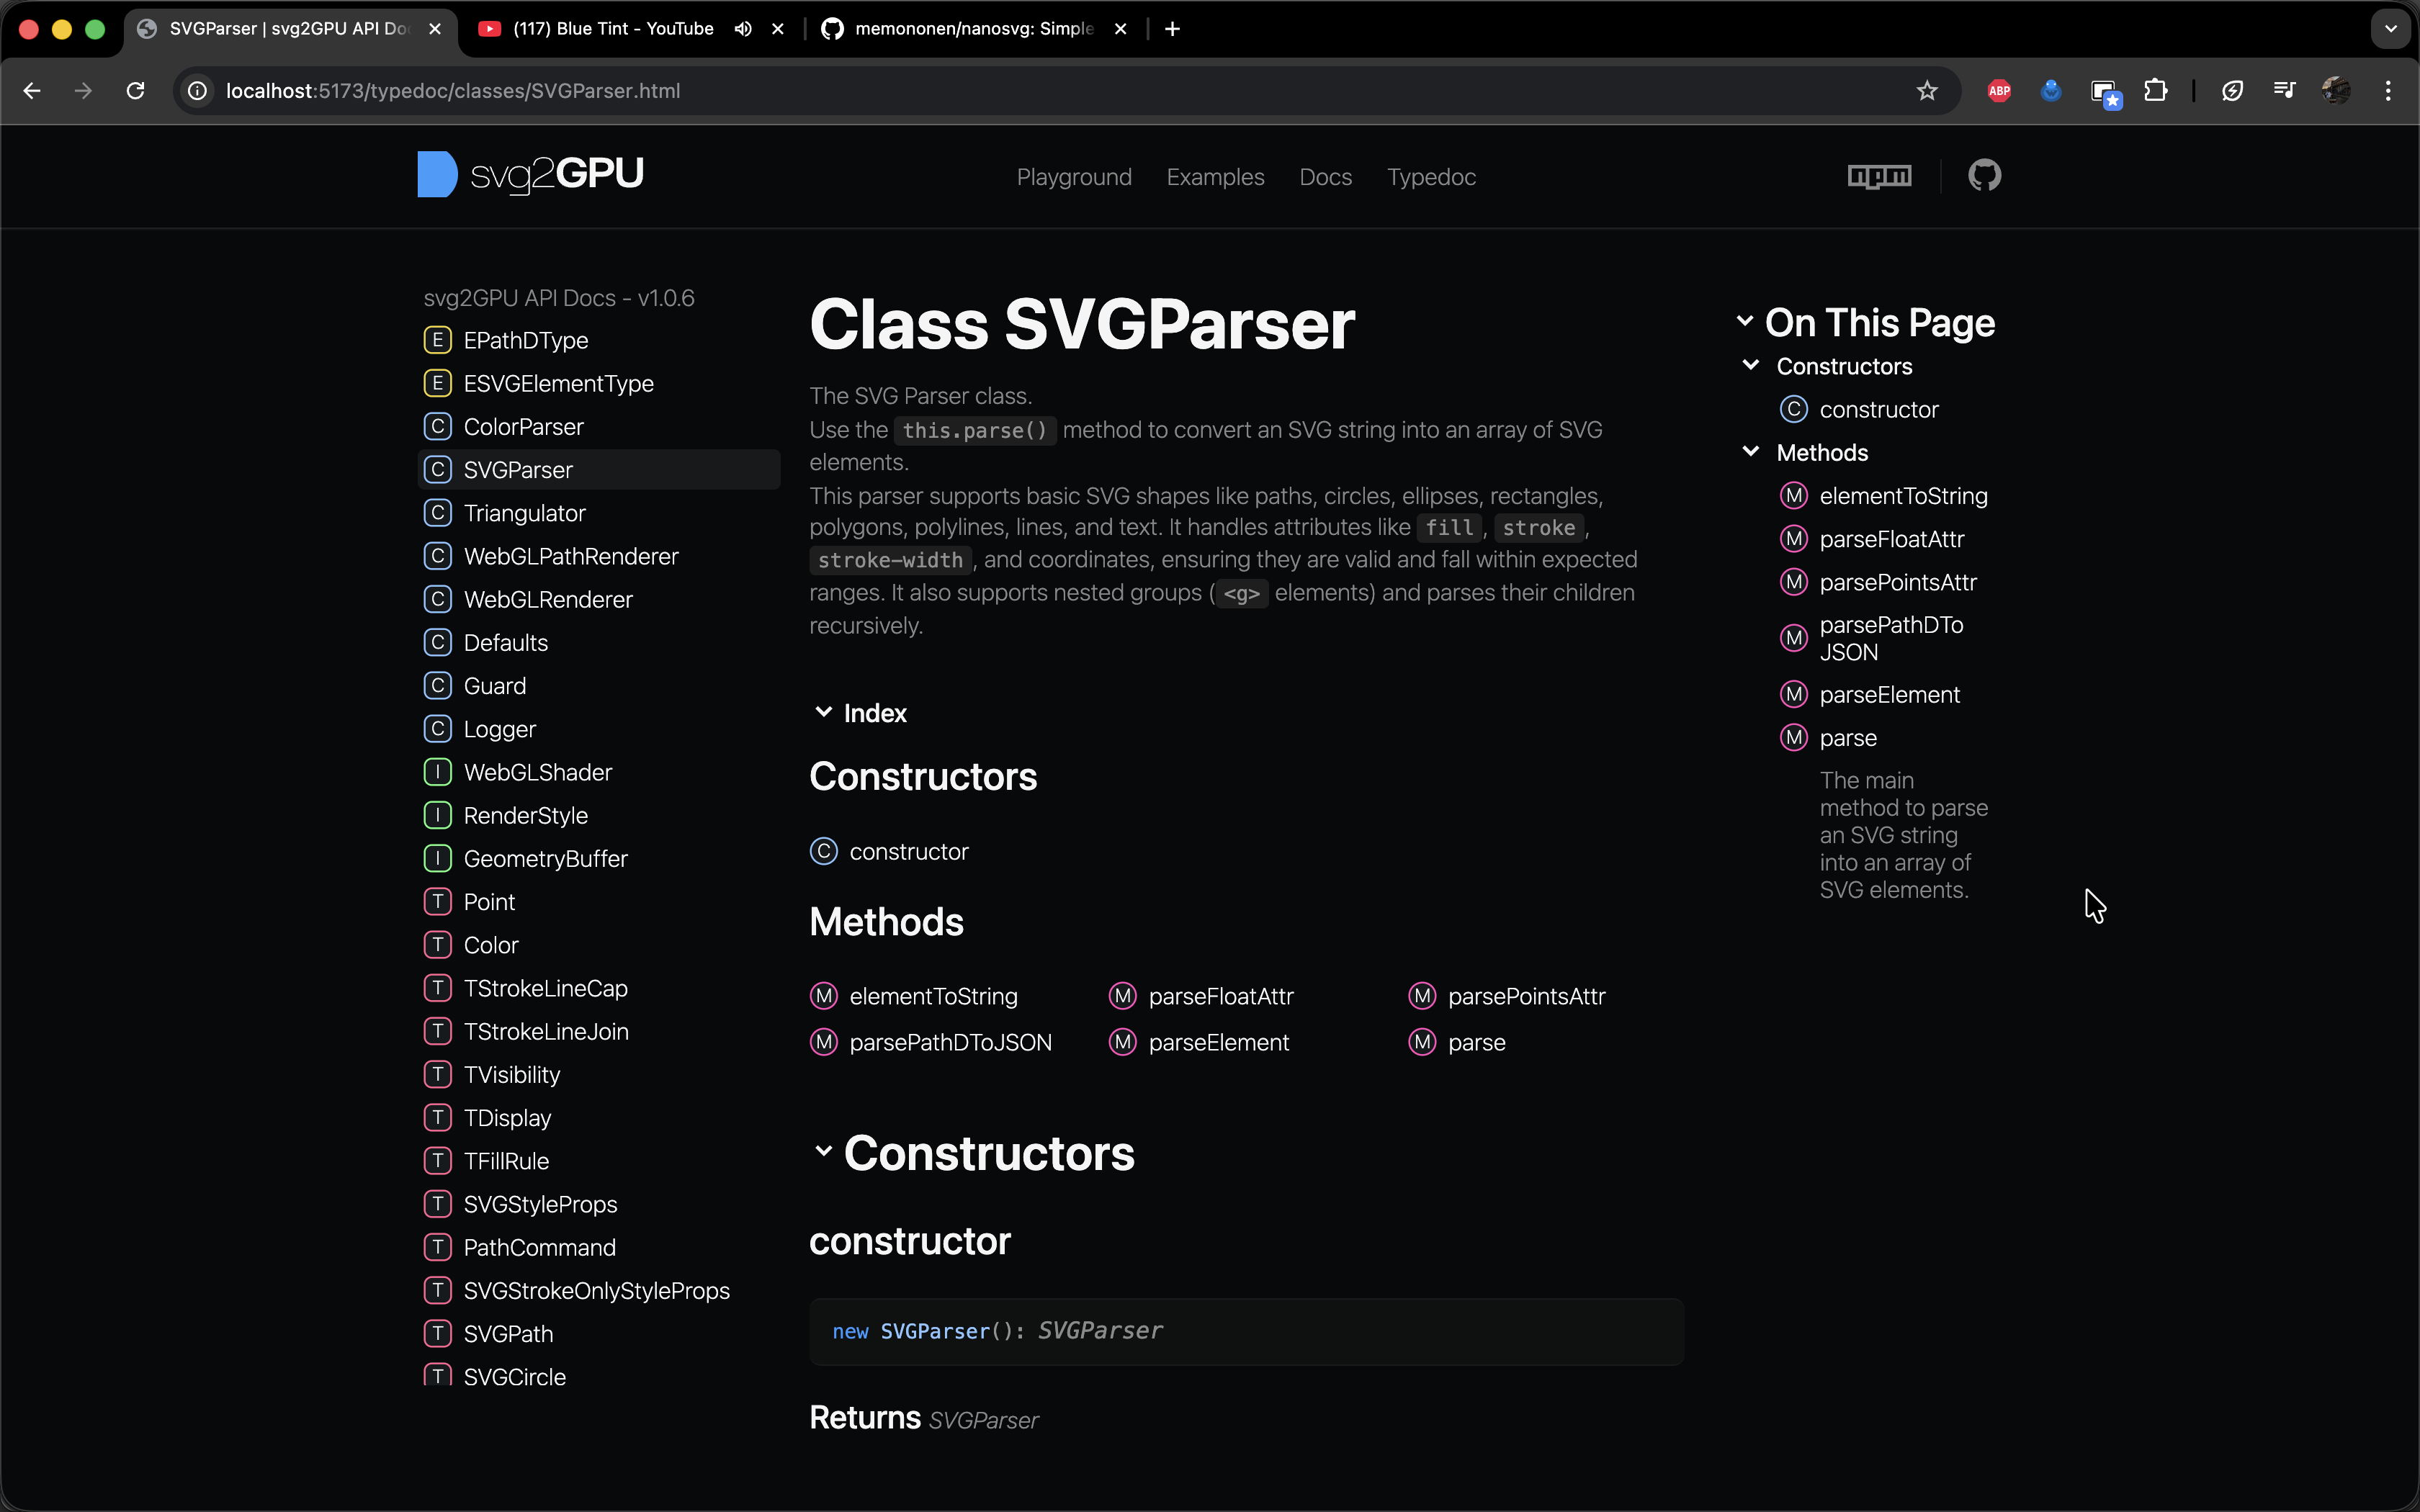
\includegraphics[width=0.92\textwidth]{figures/Typedoc.png}
    \caption{TypeDoc-generated API documentation integrated in the project workflow}
    \label{fig:typedoc_compact}
\end{figure}

\section{Implementation traceability}

\begin{table}[htbp]
\centering
\caption{Compact traceability matrix}
\label{tab:traceability_compact}
\begin{tabular}{>{\raggedright\arraybackslash}p{1.6cm} >{\raggedright\arraybackslash}p{5.4cm} >{\raggedright\arraybackslash}p{5.8cm}}
\toprule
\textbf{ID} & \textbf{Target} & \textbf{Implemented evidence} \\
\midrule
F1 & SVG parse pipeline for path-based input & typed command parsing + dedicated executable tests \\
F2 & style and color normalization & color parser tests + normalized style fields in parsed elements \\
F3 & render-ready geometry flow & path-to-geometry and stroke conversion in renderer pipeline \\
F4 & interactive validation & playground editor, previews, and diagnostics \\
F5 & API discoverability & TypeDoc-generated reference pages \\
\bottomrule
\end{tabular}
\end{table}

\section{Operational data flow}

At runtime, modules cooperate through explicit data hand-offs.
A compact operational sequence is:

\begin{enumerate}
\item source SVG is validated and parsed into typed elements,
\item style fields are normalized into canonical values,
\item conversion routines produce geometry arrays,
\item renderer uploads arrays and issues draw calls,
\item diagnostics are surfaced to the client console/log channel.
\end{enumerate}

This data flow minimizes hidden state and helps keep behavior reproducible.
It also makes instrumentation straightforward when profiling or extending the system.

\subsection{Operational checkpoints and quality gates}

The implementation keeps lightweight quality gates between major stages.
These gates are not expensive verification passes, but small checks that prevent invalid state propagation.
In practice, they include mandatory-field validation before command parsing, finite-value checks before buffer generation, and renderer-side checks before issuing draw calls.

This checkpoint strategy has two practical benefits.
First, it reduces debugging time because the first failing gate identifies the most likely layer where data became invalid.
Second, it improves maintainability by making contract violations explicit instead of silently corrected.
For a thesis prototype, this behavior is preferable because it favors predictability and transparency over implicit recovery heuristics.

\section{Limitations and engineering trade-offs}

The implementation intentionally prioritizes robustness and modularity over full feature breadth.
Current limitations include partial SVG coverage, evolving triangulation depth for difficult contours, and WebGL-first practical execution.
These are acceptable for the thesis scope and keep the architecture extensible.

An additional trade-off is deliberate avoidance of over-optimization before behavior stabilization.
The implementation prefers predictable results and explicit diagnostics first, then optimization opportunities (buffer reuse, batching, algorithm upgrades) as a second phase.

\section{Chapter summary}

This chapter mapped theory to implementation.
\texttt{Svg2GPU} is realized as a modular system with explicit parser contracts, conversion flow, rendering integration, and developer-facing tooling.
The result is a technically coherent prototype that supports both functional use and structured evaluation.
